\begin{figure}[h!]
    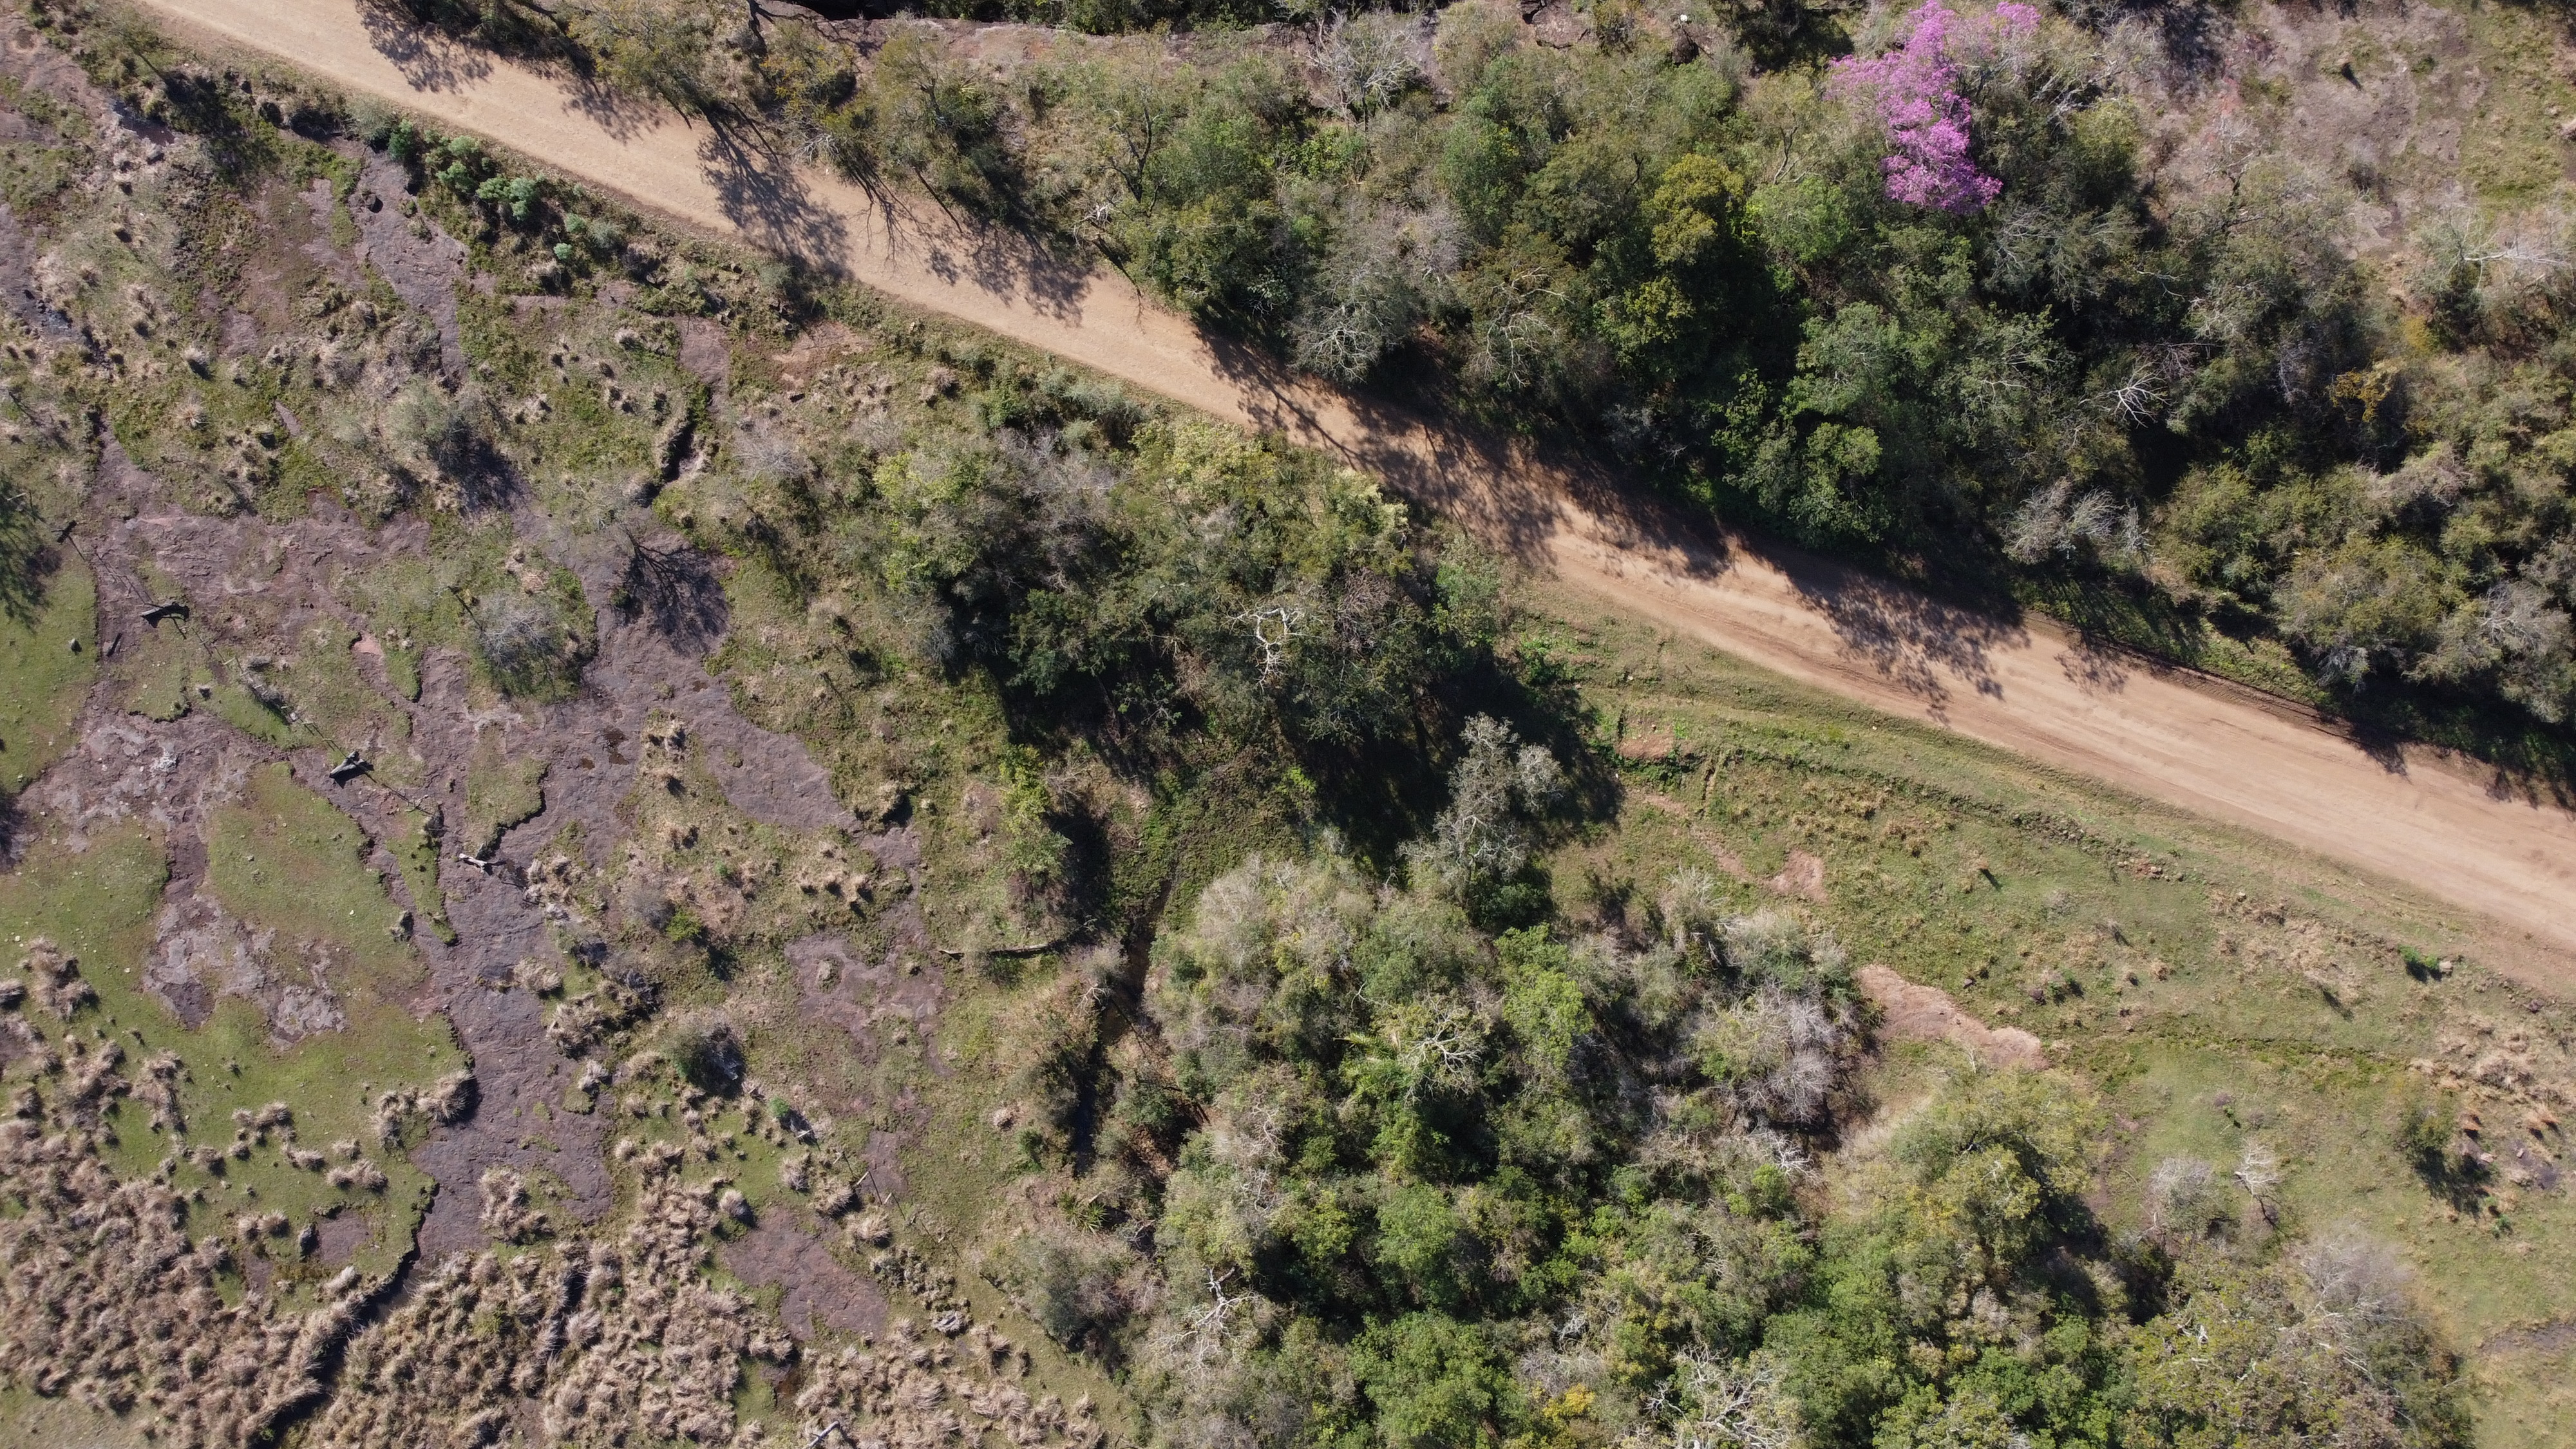
\includegraphics[width=\textwidth]{Imagenes/street.jpg}
     \hfill
     \caption{Escena capturada con pocos árboles}
    \label{calle}
\end{figure}

\begin{figure}[h!]
    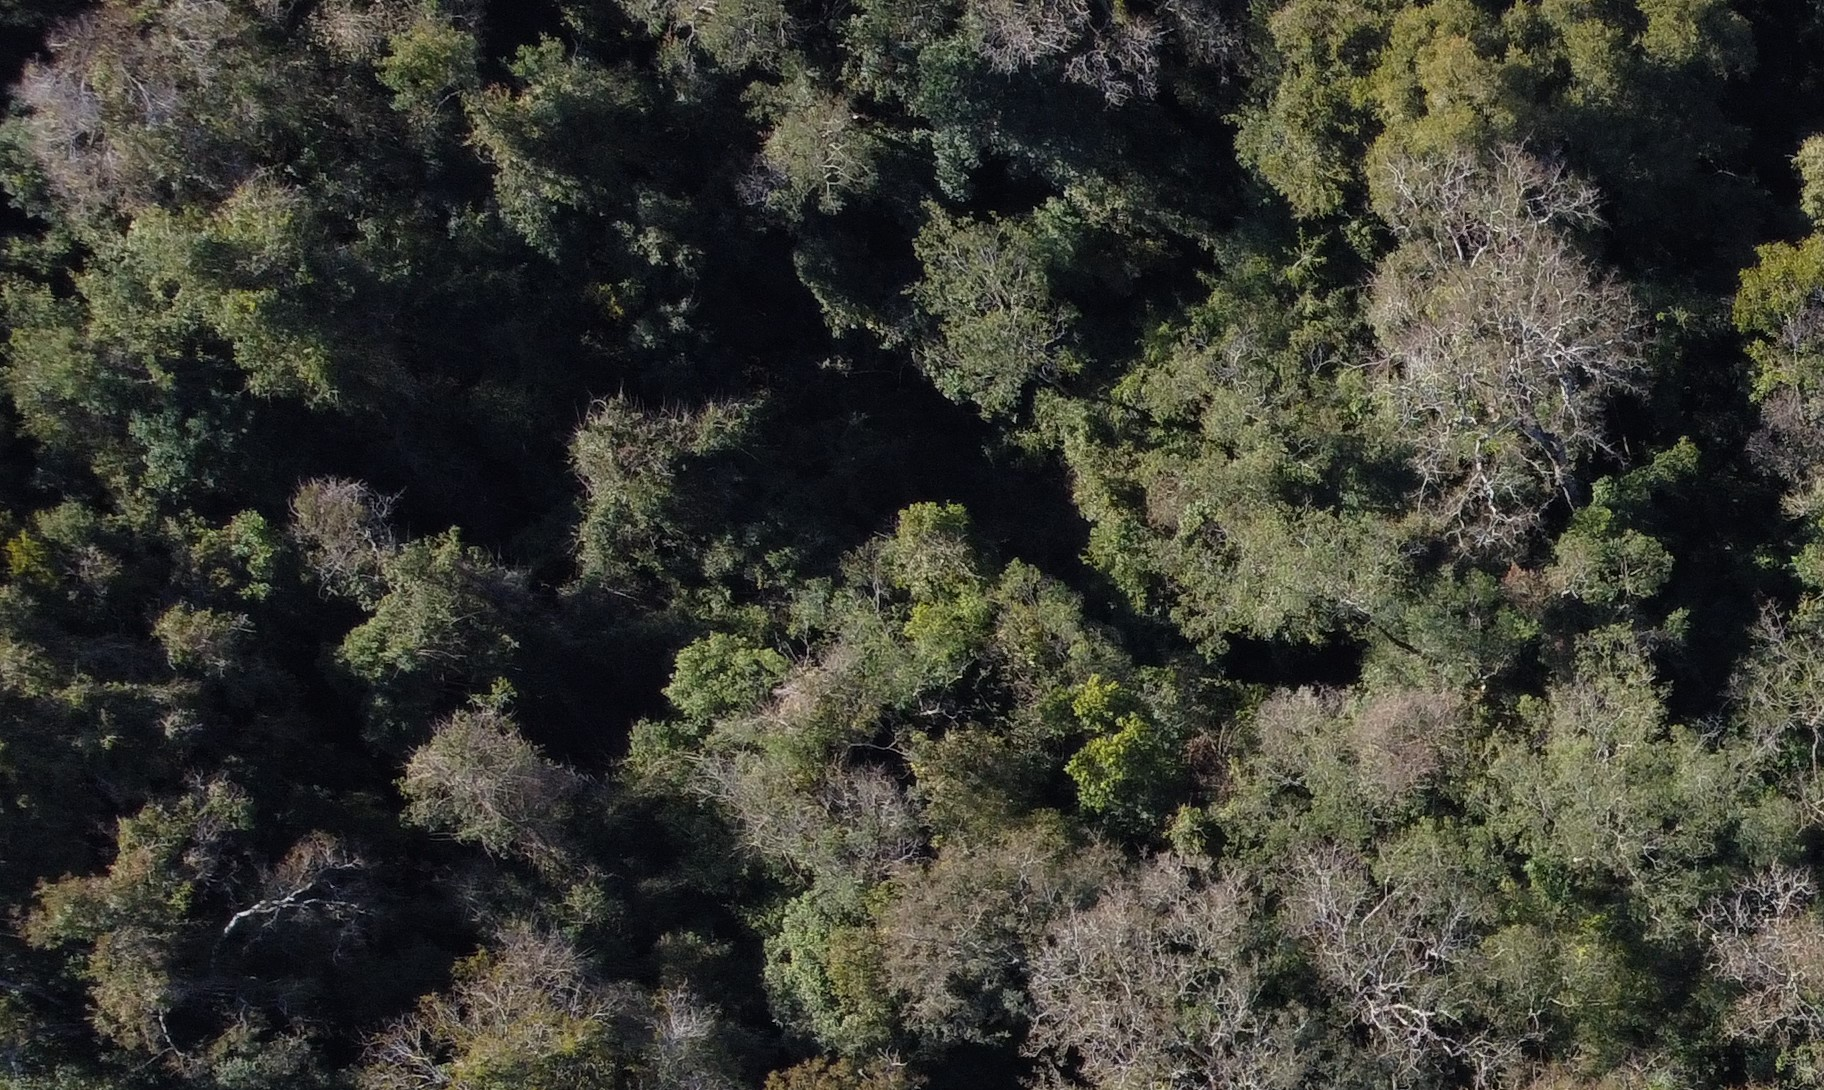
\includegraphics[width=\textwidth]{Imagenes/dense canopy.jpg}
     \hfill
     \caption{Escena capturada con dosel tupido}
    \label{tupido}
\end{figure}


\begin{figure}[h!]
    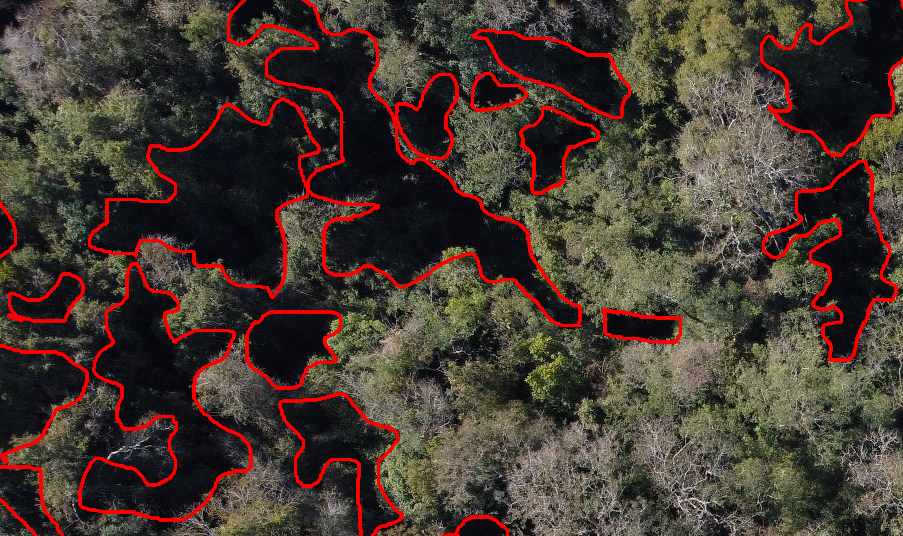
\includegraphics[width=\textwidth]{Imagenes/contours.png}
     \hfill
     \caption{Contornos de sombras en dosel tupido}
    \label{contorno1}
\end{figure}

\begin{figure}[h!]
    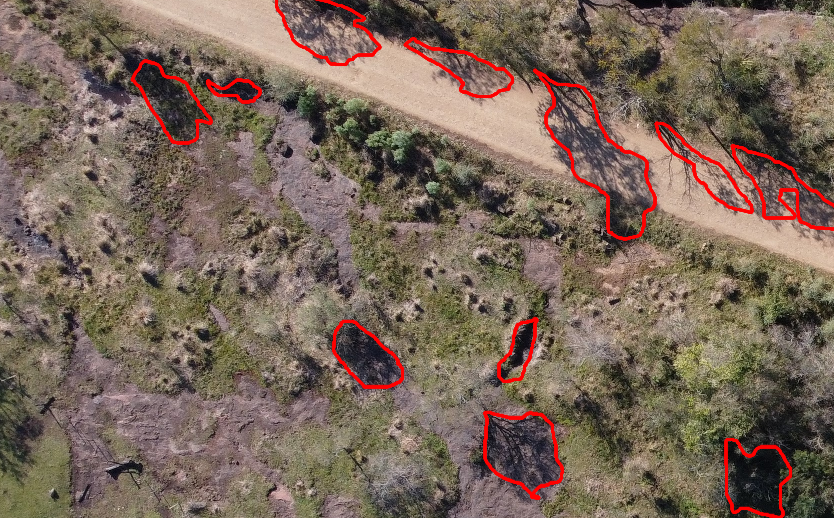
\includegraphics[width=\textwidth]{Imagenes/contours2.png}
     \hfill
     \caption{Contorno de sombras en imagen con pocos árboles}
    \label{contorno2}
\end{figure}

\begin{figure}[h!]
     \centering
     \begin{subfigure}[b]{0.5\textwidth}
         \centering
         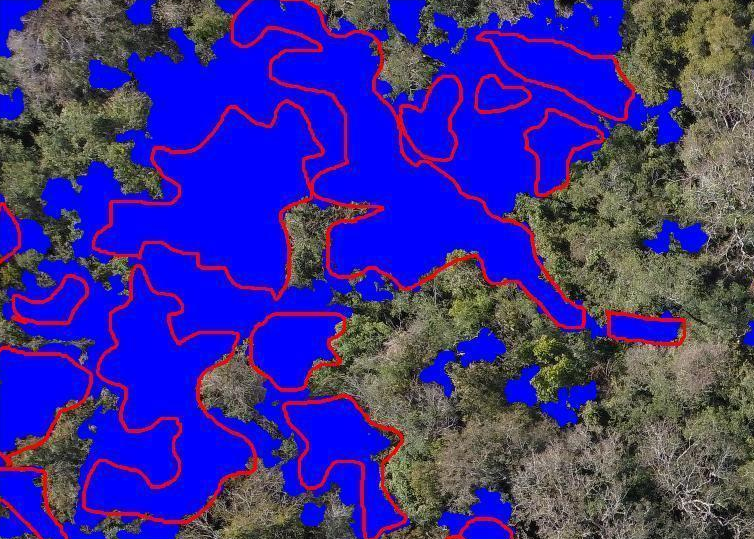
\includegraphics[width=\textwidth]{Imagenes/superposition of masks.png}
         \caption{Percentil 60º}
         \label{p60}
     \end{subfigure}
     \hfill
     
     \begin{subfigure}[b]{0.5\textwidth}
         \centering
         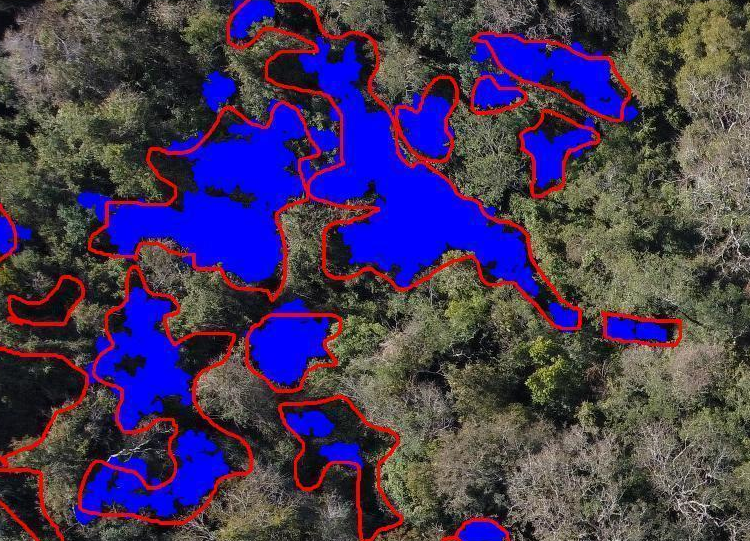
\includegraphics[width=\textwidth]{Imagenes/superposition of masks 2.png}
         \caption{Percentil 85º}
         \label{p85}
     \end{subfigure}
        \caption{Superposición de máscaras automática y manual}
        \label{superposicion}
\end{figure}

\begin{figure}[h!]
    \centering
  \begin{subfigure}[b]{\textwidth}
    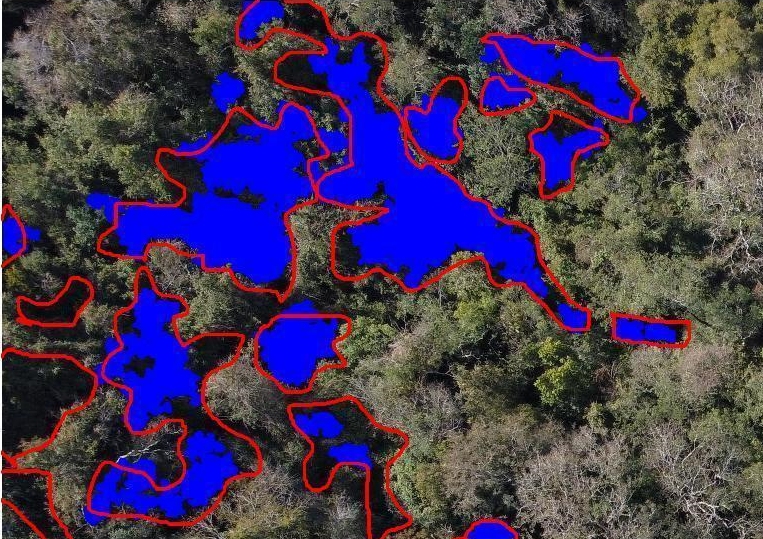
\includegraphics[width=\textwidth]{Imagenes/blue minus red 85.png}
     \hfill
     \caption{\textpsi\textsubscript{BR}}
    \label{azulrojo}
 \end{subfigure}

 \begin{subfigure}[b]{\textwidth}
    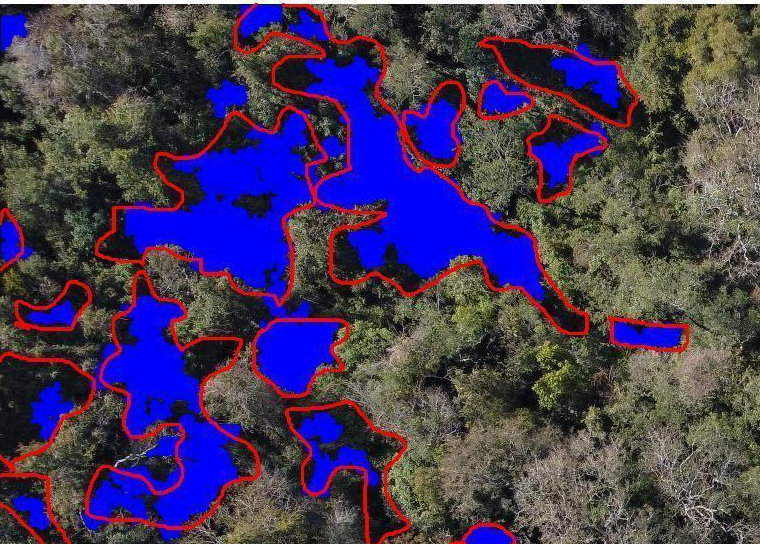
\includegraphics[width=\textwidth]{Imagenes/blue minus green 85.png}
     \hfill
     \caption{\textpsi\textsubscript{BG}}
    \label{azulverde}
 \end{subfigure}

 \begin{subfigure}[b]{\textwidth}
    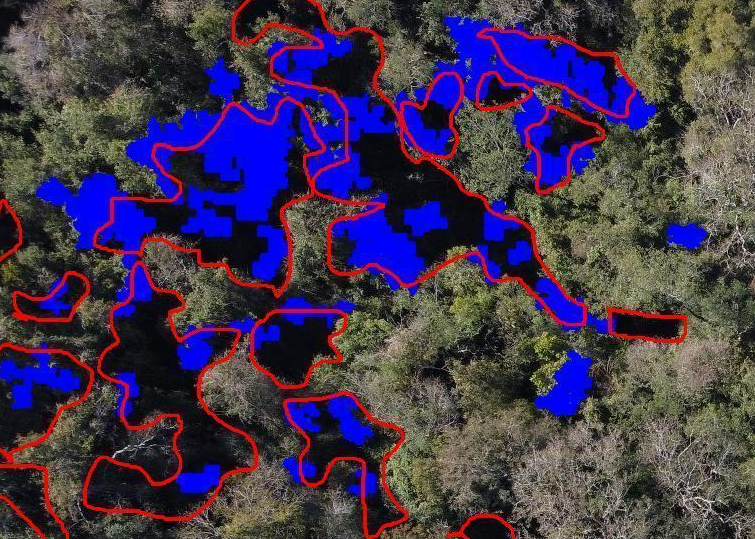
\includegraphics[width=\textwidth]{Imagenes/green minus red 85.png}
     \hfill
     \caption{\textpsi\textsubscript{GR}}
    \label{verderojo}
 \end{subfigure}
 \caption{Superposición de máscaras automática y manual}
        \label{p85BRBGGR}
\end{figure}

\begin{figure}[h!]
    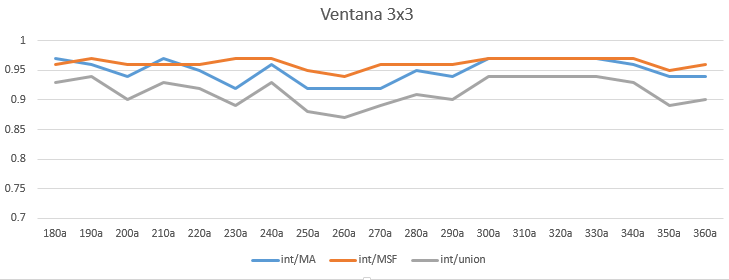
\includegraphics[width=\textwidth]{Imagenes/filter 3x3.png}
     \hfill
     \caption{Filtro 3x3}
    \label{filter3x3}
\end{figure}

\begin{figure}[h!]
    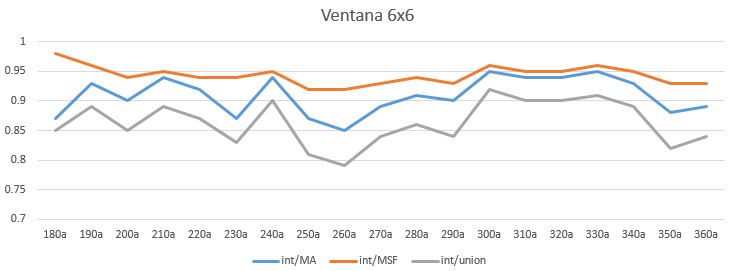
\includegraphics[width=\textwidth]{Imagenes/filter 6x6.png}
     \hfill
     \caption{6x6}
    \label{filter6x6}
\end{figure}

\begin{figure}[h!]
    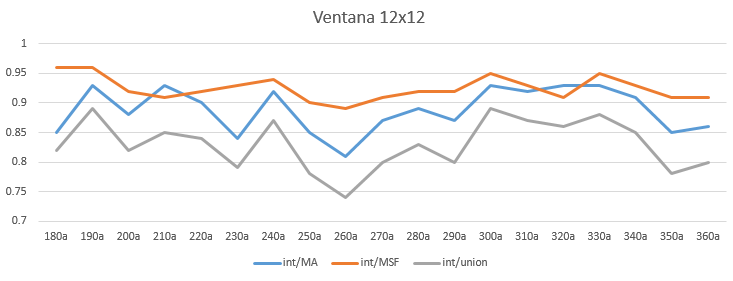
\includegraphics[width=\textwidth]{Imagenes/filter 12x12.png}
     \hfill
     \caption{12x12}
    \label{filter12x12}
\end{figure}